% WIFI
\subsection{IEEE 802.11 --- Wi-Fi}%
\label{sec:wifi}
IEEE 802.11, commonly known as Wi-Fi, is part of the IEEE 802 set of \gls{lan} protocols, and specifies the set of \gls{mac2} and
physical layer protocols for implementing \gls{wlan}
communication in a wide sprectrum of frequencies, ranging from 2.4--60 GHz.

\subsubsection{TCP/IP}%
\label{sec:tcpip}
The most commonly used protocols for Internet communications, including Wi-Fi,
are \gls{tcp} and \gls{ip}, usually associated together, being part of the \gls{osi} model
(Fig.~\ref{fig:osi-model}), which characterises and standardises the
communication functions of a telecommunication or computing system, being
agnostic to their underlying internal structure and technology.

A computer protocol is a standardised procedure for the exchange and
transmission of data between devices, as requested for the application processes.
The TCP provides services at the Transport layer, handling the reliable, unduplicated
and sequenced delivery of data~\cite{carne2004professional}, while the UDP provides data transportation
without guaranteed data delivery or acknowledgments. The TCP can be thought of
a reliable version of \gls{udp}, generalizing. The IP part of the TCP/IP suite, providing
services at the Network layer, is used to make origin and destination addresses
available to route data across networks.

These protocols are applied in sequence to the user's data to create a frame
that can be transmitted from the sending application to the receiving
application.
The receiver reverses the procedure to obtain the original user’s data and pass
them to the receiving application~\cite{carne2004professional}.

Another interesting fact, due to the technology agnostic aspect of the OSI
Model, is that IP and the higher-level protocols may be implemented on several
kinds of physical nets.
% OSI model
\begin{figure}[!hbt]
\centering
    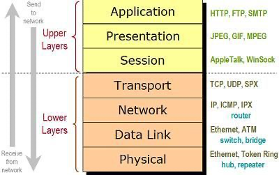
\includegraphics[width=0.5\textwidth]{./img/osi-model.png}
  \caption{\gls{osi} model}%
\label{fig:osi-model}
\end{figure}
%%% Local Variables:
%%% mode: latex
%%% TeX-master: "../../../dissertation"
%%% End:
